Assuming that we have a correct half adder circuit, we will construct a full adder circuit. The following box below describes how to add 3 one bit numbers $p$, $q$, and $r$.

If you are a little confused by this description, try to keep in mind that we are really just doing normal addition, just in binary.
\begin{tcolorbox}
We want to add the three bits $p$, $q$, and $r$. First we will add the two bits $p$ and $q$. We will get something like 
\[p + q = c_1s_1\]
where $c_1$ and $s_1$ are bits in binary. The half adder we made will compute these two bits.

After this, we add $r$ to $s_1$ to get $c_2s_2$. To finish off, we add the two carry bits $c_1$ and $c_2$ to get a value $c$. Then the final result of the full adder is $cs_2$. Note that adding $3$ one bit numbers will not get you a number longer than $2$ bits.
\end{tcolorbox}
\begin{enumerate}
    \item Explain why in this process, the two carry bits $c_1$ and $c_2$ cannot be both $1$. This is why when combining $c_1$ and $c_2$ at the end it suffices to use an OR gate instead of an XOR gate.

    \item Based on the information in the box and the considerations of part i), construct the full adder circuit having ``black-boxed'' the half-adder circuit, as in figure \ref{fig:my_label}
    
    \begin{figure}[ht]
        \centering
        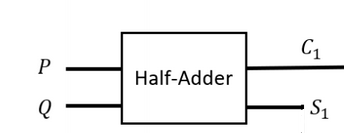
\includegraphics{Ch2/003.PNG}
        \caption{Black boxed half-adder}
        \label{fig:my_label}
    \end{figure}
    
    \item How many AND, OR, and NOT gates does this construction use? (The half adder we will be considering uses $2$ AND gates, one OR gate, and one NOT gate.)
\end{enumerate}